\section{Технический проект}

\subsection{Общая характеристика организации решения задачи}
Обсуждение методологии разработки, включая Agile подходы, планирование спринтов и процессы контроля качества.

\subsection{Обоснование выбора технологий проектирования}
\subsubsection{.NET Core}
Обоснование выбора .NET Core для серверной разработки: производительность, масштабируемость и кросс-платформенность.
Начиная с версии .NET core 6.0, которая была выбрана для разработки, поддерживается работа с админ-панелью "из коробки", что позволяет сэкономить ресурсы на ращработки панели администратора.
\subsubsection{Entity Framework Core}
Entity Framework Core является ORM (Object-Relational Mapping) для .NET Core. Он позволяет работать с базами данных, используя объектно-ориентированный подход. Entity Framework Core позволяет работать с различными СУБД, в том числе с PostgreSQL, которая была выбрана для разработки.
\subsubsection{Angular}
Angular является самым строгим и требовательным к архитектуре среди других Frontend библиотек. Такие свойства Angular делают его идеальным инструментом для разработки сложных масштабируемых приложений. Мощные инструменты для создания интерактивных интерфейсов и легкость интеграции с REST API.
\subsection{Архитектура программной системы}
Взаимодействие между .NET Core и Angular через REST API, использование PostgreSQL для хранения данных.

\subsection{Компоненты программной системы}
Детальное описание компонентов системы на .NET Core и Angular, их функций и взаимодействия.

\subsection{Проект данных программной системы}
\subsubsection{Описание сущностей серверной части}
Структура базы данных, связи, индексы и использование Entity Framework Core.
\subsubsection{Описание сущностей клиентской части}
Структура данных на клиенте, API взаимодействия и обработка ответов.

\subsection{Проектирование пользовательского интерфейса}
Процесс проектирования UI/UX, создание макетов, прототипирование, тестирование интерфейса и адаптивный дизайн.

\subsection{Диаграмма компонентов и схема обмена данными между файлами компонента}

Диаграмма компонентов описывает особенности физического представления разрабатываемой системы. Она позволяет определить архитектуру системы, установив зависимости между программными компонентами, в роли которых может выступать как исходный, так и исполняемый код. Основными графическими элементами диаграммы компонентов являются компоненты, интерфейсы, а также зависимости между ними. На рисунке \ref{comp:image} изображена диаграмма компонентов для проектируемой системы. Она включает в себя сервер с операционной системой, на которой установлена система управления содержимым, включающая в себя базу данных и интерфейс. Помимо этого на диаграмме изображен клиентский компьютер с операционной системой, на которой установлен браузер.

\begin{figure}[ht]
\center{\includegraphics[width=1\linewidth]{comp}}
\caption{Диаграмма компонентов}
\label{comp:image}
\end{figure}

% Любой компонент должен быть вызван в сценарии страницы web-сайта. Web-страница передает данные компоненту в момент вызова последнего.
%
% На рисунке \ref{data:image} представлена схема обмена данными между сценариями компонента при вызове компонента на странице сайта.
%
% \begin{figure}[ht]
% \center{\includegraphics[width=1\linewidth]{data}}
% \caption{Диаграмма компонентов}
% \label{data:image}
% \end{figure}
%
% При вызове компонента в сценарии web-страницы указываются значения параметров компонента, которые далее посредством массива \$arParams передаются в сценарий файла component.php.
%
% В сценарии файла component.php посредством метода \linebreak IncludeComponentTemplate класса CBitrixComponent происходит вызов одного из шаблонов компонента. Id шаблона также определяется в сценарии страницы web-приложения и неявно для разработчика передается указанный выше метод. Подключается сценарий файла template.php одного из шаблонов, в который передается, возможно, измененный в сценарии component.php массив \$arParams и, также, сформированный в сценарии component.php массив \$arResult. Оба этих массива доступны также и в файле result\_modifier.php, который подключается перед подключением файла template.php.
%
% Работа компонента заканчивается в момент завершения работы сценария файла component.php, т.е. возможно выполнить действия уже после подключения шаблона. Однако, если массив \$arResult будет изменен в сценарии шаблона, в сценарий файла компонента component.php измененные данные переданы не будут.

\subsection{Диаграмма размещения}

Диаграмма размещения (рис.~\ref{place:image}) отражает физические взаимосвязи между программными и аппаратными компонентами системы.

\begin{figure}[ht]
\center{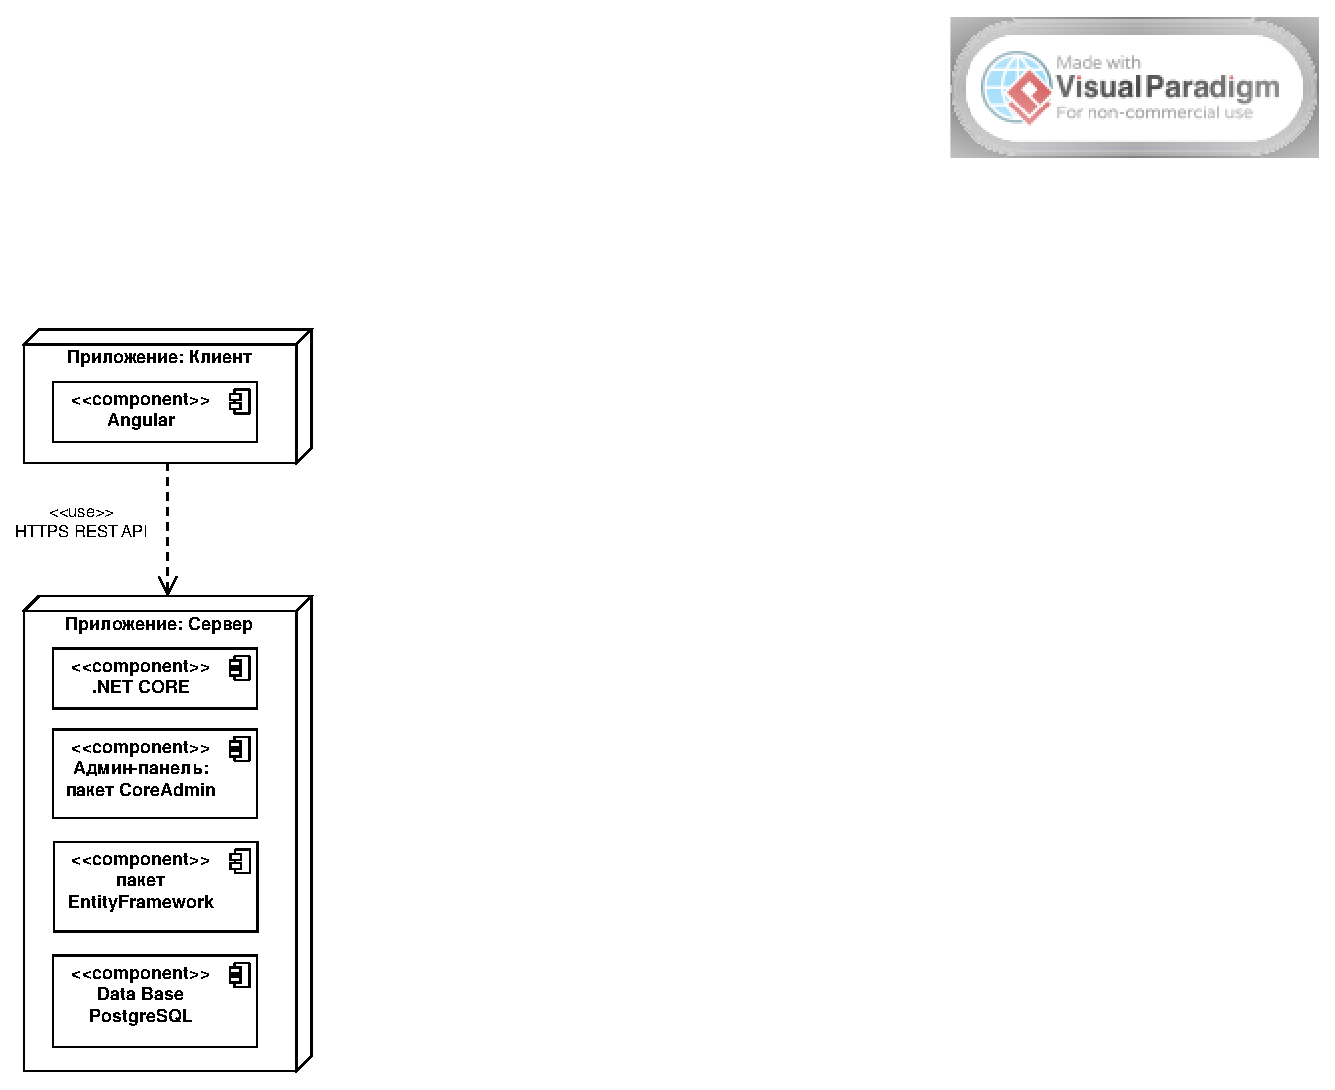
\includegraphics[width=1\linewidth]{client-server.eps}}
\caption{Диаграмма размещения}
\label{client-server.eps:image}
\end{figure}

Она является хорошим средством для показа маршрутов перемещения объектов и компонентов в распределенной системе.

В таблице \ref{ssevsws:table} приведен пример использования пакета xltabular с автоматическим расчетом ширины столбца.

\begin{xltabular}{\textwidth}{|c|X|X|}
	\caption{Сравнение протоколов SSE и WebSocket\label{ssevsws:table}}\\ \hline
	~  & \centrow  SSE & \centrow WebSocket \\ \hline
	\endfirsthead
	\continuecaption{Продолжение таблицы \ref{ssevsws:table}}
	~ & \centrow SSE & \centrow WebSocket \\ \hline 
	\finishhead
	Направленность & 
	Однонаправленный, полудуплексный: данные посылает только сервер & 
	Двунаправленный, полнодуплексный: и сервер, и клиент могут обмениваться сообщениями \\ \hline 
	Соединение  & HTTP & WS \\ \hline 
	Тип данных & Только текст & Бинарные и текстовые данные \\ \hline 
	Доп. возможности & Встроенный механизм идентификаторов событий и переподключения & Переподключение и идентификация события реализуются на стороне приложения
\end{xltabular}

\subsection{Содержание информационных блоков. Основные сущности}

Проанализировав требования, можно выделить шесть основных сущностей:
\begin{itemize}
\item "<Новости">;
\item "<Продукция">;
\item "<Услуги">.
\end{itemize}

В состав сущности "<Новости"> можно включить атрибуты, представленные в таблице \ref{news:table}.

\begin{xltabular}{\textwidth}{|l|l|p{1.7cm}|X|}
	\caption{Атрибуты сущности "<Новости">\label{news:table}}\\ \hline
	\centrow Поле & \centrow Тип & \centrow Обяза\-тельное & \centrow Описание \\ \hline
	\thead{1} & \thead{2} & \centrow 3 & \centrow 4 \\ \hline
	\endfirsthead
	\continuecaption{Продолжение таблицы \ref{news:table}}
	\thead{1} & \thead{2} & \centrow 3 & \centrow 4 \\ \hline
	\finishhead
	\_id & ObjectId & true & Уникальный идентификатор \\ \hline 
	head & String & true & Заголовок новости \\ \hline 
	short & String & false & Аннотация к новости \\ \hline 
	createdAt & Date & true & Время создания новости \\ \hline 
	author & String & false & Автор новости \\ \hline 
	content & String & true & Текст новости \\ \hline 
	views & Integer & true & Количество просмотров новости зарегистрированными пользователями
\end{xltabular}

Пример использования различных типов столбцов представлен в таблице \ref{prod:table}. Рекомендуется использовать пакет xltabular для создания таблиц.

\begin{xltabular}{\textwidth}{|R|C{2.5cm}|l|T|}
	\caption{Атрибуты  сущности "<Новости разметки в LaTeX"> с использованием различных типов столбцов и многострочным заголовком\label{prod:table}}\\ \hline
	\centrow Поле & \centrow Тип & \centrow Обязательное & \centrow Описание \\ \hline
	\centrow 1 & \centrow 2 & \thead{3} & \centrow 4 \\ \hline
	\endfirsthead
	\continuecaption{Продолжение таблицы \ref{prod:table}}
	\centrow 1 & \centrow 2 & \thead{3} & \centrow 4 \\ \hline
	\finishhead
	\_id & ObjectId & true & Уникальный идентификатор \\ \hline 
	head & String & true & Заголовок новости \\ \hline 
	short & String & false & Аннотация к новости \\ \hline 
	createdAt & Date & true & Время создания новости \\ \hline 
	author & String & false & Автор новости \\ \hline 
	content & String & true & Текст новости \\ \hline 
	views & Integer & true & Количество просмотров новости зарегистрированными пользователями
\end{xltabular}

В системе предусмотрен внутренний механизм связи между разделами и элементами информационных блоков, поэтому введения дополнительных идентификаторов при реализации связей между сущностями не предполагается.

Экземпляры сущностей реализуются в информационных блоках посредством элементов, атрибуты сущности – посредством полей и свойств элемента. 
